\documentclass[a4paper,11pt]{report}
\usepackage[]{amsmath}
\usepackage[]{physics} % \bra, \ket etc
\usepackage{graphicx} %Pour les figures je crois
\usepackage{hyperref}
\usepackage[
    backend=biber, 
    natbib=true,
    style=numeric-comp,
    sorting=none, %Pour faire apparaitre les refs dans l'ordre
    hyperref=true
]{biblatex} %Imports biblatex package
\addbibresource{Bib_ch3.bib} %Import the bibliography file

\usepackage{amssymb} %quelques symboles dont gtrsim /lesssim
\usepackage{subcaption} % package pour faire des subfigures
\usepackage{multirow} % package pour multirow/multicolumn
\usepackage{booktabs} % package pour top/mid/bottom rule
\usepackage{tcolorbox} % toujours plus de boites
\usepackage{xcolor} % Pour avoir des couleurs dans les équations

\title{}
\begin{document}
\chapter{NV-NV cross-relaxations : the fluctuator model}
This chapter will cover cross-relaxations between NV centers in the non-zero magnetic field regime, both from an experimental and theoretical point of view. The case of zero magnetic field will be treated in the next chapter.

The presence of strong NV-NV dipolar interaction in dense ensemble ([NV] $\gtrsim 1\ \rm ppm$) proved to be both an obstacle for ensemble magnetometry \citep{zhou2020quantum} and an opportunity to explore and use the many-body interaction resulting from it \citep{zhou2020quantum, choi2017observation, kucsko2018critical, zu2021emergent}.

We will see in this chapter how a model of fast and slow relaxing centers, the fluctuator model \citep{choi2017depolarization}, explains most observations related to the cross-relaxation, including the stretched exponential lifetime profile and the spectral broadening of the interaction.

\section{Experimental observation of NV-NV CR}
Let us start with the experimental proof of the presence of NV-NV CR in the samples with dense NV ensembles.

When dealing with NV-NV CR, we have to make the distinction between what we will label ``equivalent" and ``non-equivalent" NV centers. Two equivalent centers are NV centers with the same spin Hamiltonian ([REF] chap 1), which implies that they both see the same transverse and longitudinal magnetic field. In contrast, non-equivalent centers are center with different single-spin Hamiltonian, which may result in different eigenstates and spin polarization for the two spins.

While the NV physics can explain cross-relaxations between non-equivalent NV centers, it cannot explain cross-relaxation between equivalent NV centers. Nevertheless, as we will see in this section, CR between both equivalent and non-equivalent NV centers is observed for samples with high NV density. 
\subsection{NV-NV CR between nonequivalent NV centers}
\label{non_equi_valent_CR}
\begin{figure}[h]
\centering
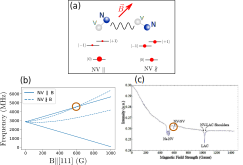
\includegraphics[width=\textwidth]{Figures/NV-NV_non_equivalent}
\caption{a) Illustration of the four possible direction of the the NV axis (four classes of NV centers) with a magnetic field along class 1 b) Representation of the polarization of two non equivalent spins, one aligned with the magnetic field (well polarized) and one misaligned with the magnetic field (unpolarized). c) Simulated frequencies for the $\ket{0} \to \ket{-1}$ and $\ket{0} \to \ket{+1}$ transitions when $\mathbf{B}\parallel [111]$ for the class aligned with B, and the 3 equivalent classes not aligned with B. d) Taken from \citep{armstrong2010nv}, PL change of an ensemble of NV centers as a magnetic field is scanned along the [111] axis.}
\label{non-equivalent NV-NV}
\end{figure}

In the absence of magnetic gradient, two NV centers can only be non-equivalent if the projection of the magnetic field upon their respective NV axis is different. Fig. \ref{non-equivalent NV-NV}-a) illustrates such a case: we label here the four possible NV axis orientation (or NV classes) 1 to 4 and we assume that the magnetic field is aligned with class 1. In this conditions, an NV center belong to class 1 will always be non-equivalent with NV centers from classes 2-4, as the projection of the magnetic field on their respective axis will never be the same. On the other hand, NV centers from the classes 2-4 are all equivalents, even though they do not necessary belong to the same class.

Fig. \ref{non-equivalent NV-NV}-b) shows the difference between the NV centers belonging to class 1 labeled NV$_\parallel$) and those belonging to classes 2-4 (labeled NV$_\nparallel$). As explained in [REF], the transverse magnetic field leads to a mixing of the eigenstates \footnote{The states of the misaligned NV on Fig. \ref{non-equivalent NV-NV}-b) are labeled $\ket{0},\ket{\pm 1}$ which is an abusive (but common) notation since the mixing caused by the transverse field means that the eigenstates of $S_z$ are no longer the Hamiltonian eigenstates.} and to a loss of the optical polarization mechanism. As a result, the NV$_\nparallel$ spins are less polarized than the NV$_\parallel$ ones, which is a necessary condition to observe cross-relaxation.

Another necessary condition to observe cross-relaxation is the condition of co-resonance. In most situations, non-equivalent NV centers are not co-resonant, as the differences in the spin Hamiltonian generally leads to different eigenvalues. This is in contrast with equivalent NV centers which are by definition always resonant. Fig. \ref{non-equivalent NV-NV}-c) shows the transition frequencies of spin from class 1 and a spin from class 2-4 as a function of the magnetic field amplitude. Unintuitively, there is a co-resonance between the two $\ket{0} \to \ket{+1}$ transitions for $\abs{\mathbf{B}}=592\ \rm G$. For this particular value of the magnetic field, cross-relaxation between the NV centers from class 1 and those from classes 2-4 is possible.

Finally, Fig. \ref{non-equivalent NV-NV}-d), which was presented in the last chapter, shows the experimental value of the total NV PL as a function of the magnetic field amplitude, in a scenario similar to the one we just described. We can indeed observe the signature of NV-NV CR in the presence of a PL dip at $\abs{\mathbf{B}}=592\ \rm G$.

As previously mentioned, cross-relaxation between non-equivalent NV centers is easily explained by the physics of single NV centers, and has been known for more than thirty years \citep{holliday1989optical, van1989cross}.

\subsection{NV-NV CR between equivalent NV centers}

\begin{figure}[h]
\centering
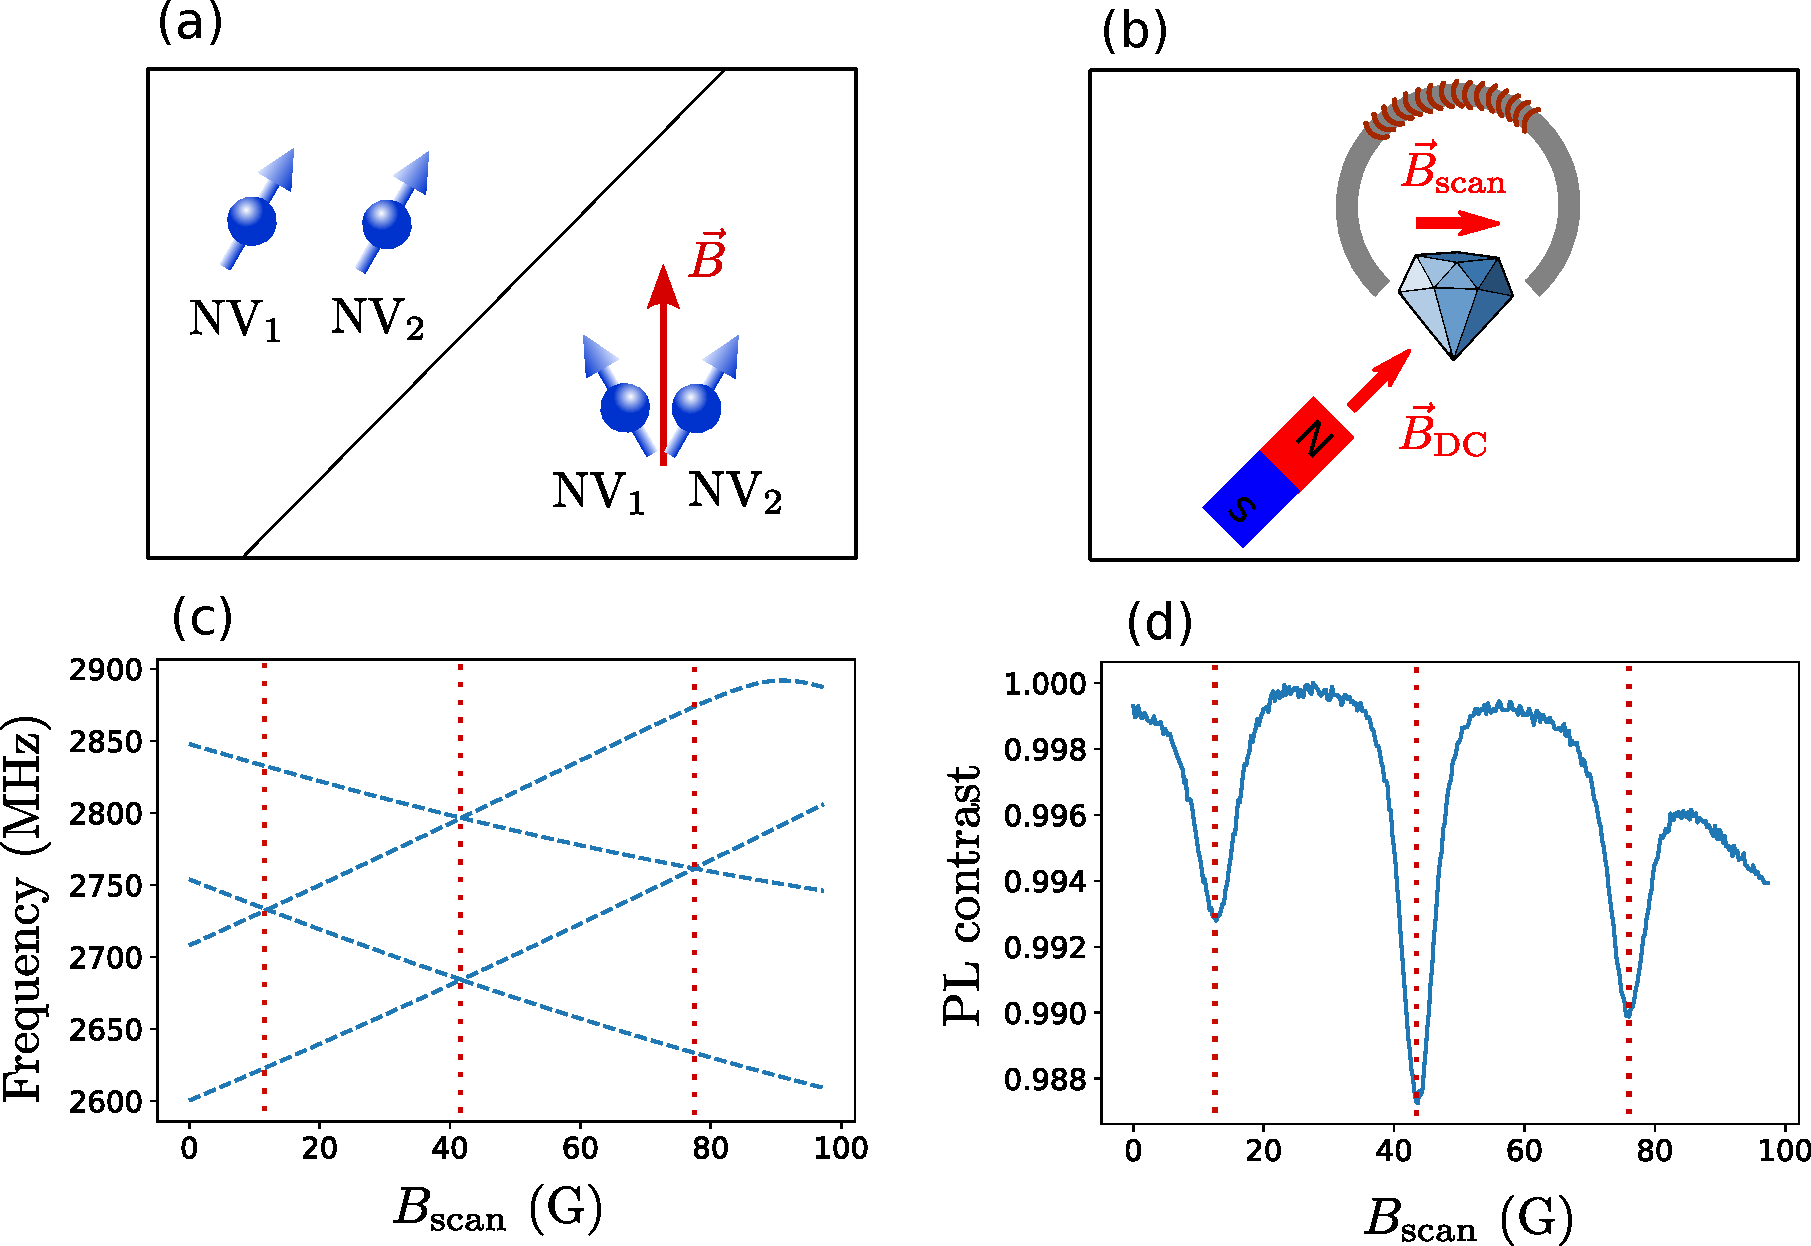
\includegraphics[width=\textwidth]{Figures/NV-NV_equivalent}
\caption{CR between equivalent NV centers for sample ADM-15-1. (a) Representation of equivalent NV centers: either two NVs from the same class, or two classes with the same projected magnetic field. (b) Magnetic setup used for the experiment: a permanent magnet is used to apply a bias magnetic field, and an electromagnet is used to add a variable magnetic field. (c) Simulation showing the $\ket{0}\to\ket{-1}$ transition frequencies for the 4 classes of NV centers as a function of the scanned magnetic field. The transitions were computed based on ODMR spectra recorded for different magnetic field values. (d) Change in the PL of the NV centers ensemble as a function of the scanned magnetic field.}
\label{equivalent NV-NV}
\end{figure}

More recently, experiments on dense NV ensemble ($[\rm NV ] >1\ \rm ppm$) or at low temperature have shown that there were cross-relaxations even between equivalent NV centers \citep{jarmola2012temperature, mrozek2015longitudinal, jarmola2015longitudinal, choi2017depolarization}.

Fig. \ref{equivalent NV-NV}-a) illustrates the two possible scenarios for equivalent NV centers: either two NVs from the same class, or two NVs from different classes with the same projection of the magnetic field upon their respective axis (i.e. $\mathbf{B}$ belongs to the plane of mirror symmetry of the two spins). 

In the second case, by moving the magnetic field in and out of the symmetry plane, we can change the resonance condition between the two NV classes and measure the contribution of NV-NV cross-relaxation to the NV PL and spin lifetime. To do so, we need to add an initial bias magnetic field in addition to the scanned magnetic field, as represented in Fig. \ref{equivalent NV-NV}-b). %When doing so, the magnetic field felt by the diamond won't have a fixed orientation during the scan, and when the magnetic field crosses certain crystalline planes (detailed below), its projection on two or more classes of NV centers will be the same.

Fig. \ref{equivalent NV-NV}-c) shows the transition frequencies of the $\ket{0}\to\ket{-1}$ transition for the 4 classes of NV centers on sample ADM-15-1, an HPHT micro-diamond with $[\rm NV]\sim 3\ \rm ppm$. There are three magnetic field values $B_{\rm scan} \approx$ 12, 42 and 77 G for which there is an inter-class resonance. These values are reported in the figure with red dotted lines. Unlike the case presented in Fig. \ref{non-equivalent NV-NV}, all the inter-class resonances reported in Fig. \ref{equivalent NV-NV}-c) are between equivalent classes.

Finally, Fig. \ref{equivalent NV-NV}-d) shows the PL contrast as the electromagnet field is scanned. There are 3 very clear dips when $B_{\rm scan} \approx$ 12, 42 and 77 G which coincide with inter-class resonances. We will see later that this PL dip is associated with a decrease of the NV centers spin $T_1$ time from both classes.

This observation, and similar ones made by many groups \citep{jarmola2012temperature, mrozek2015longitudinal, choi2017depolarization, akhmedzhanov2017microwave, giri2018coupled}, seem to indicate that there are CR between equivalent NV centers. This is however incompatible with our previous assumptions that equivalent NV centers are equally polarized and bright. To understand this phenomenon, we will need to introduce new hypotheses.

\section{NV inhomogeneity and the fluctuator model}

\subsection{CR in an inhomogeneous NV bath}
\begin{figure}[h]
\centering
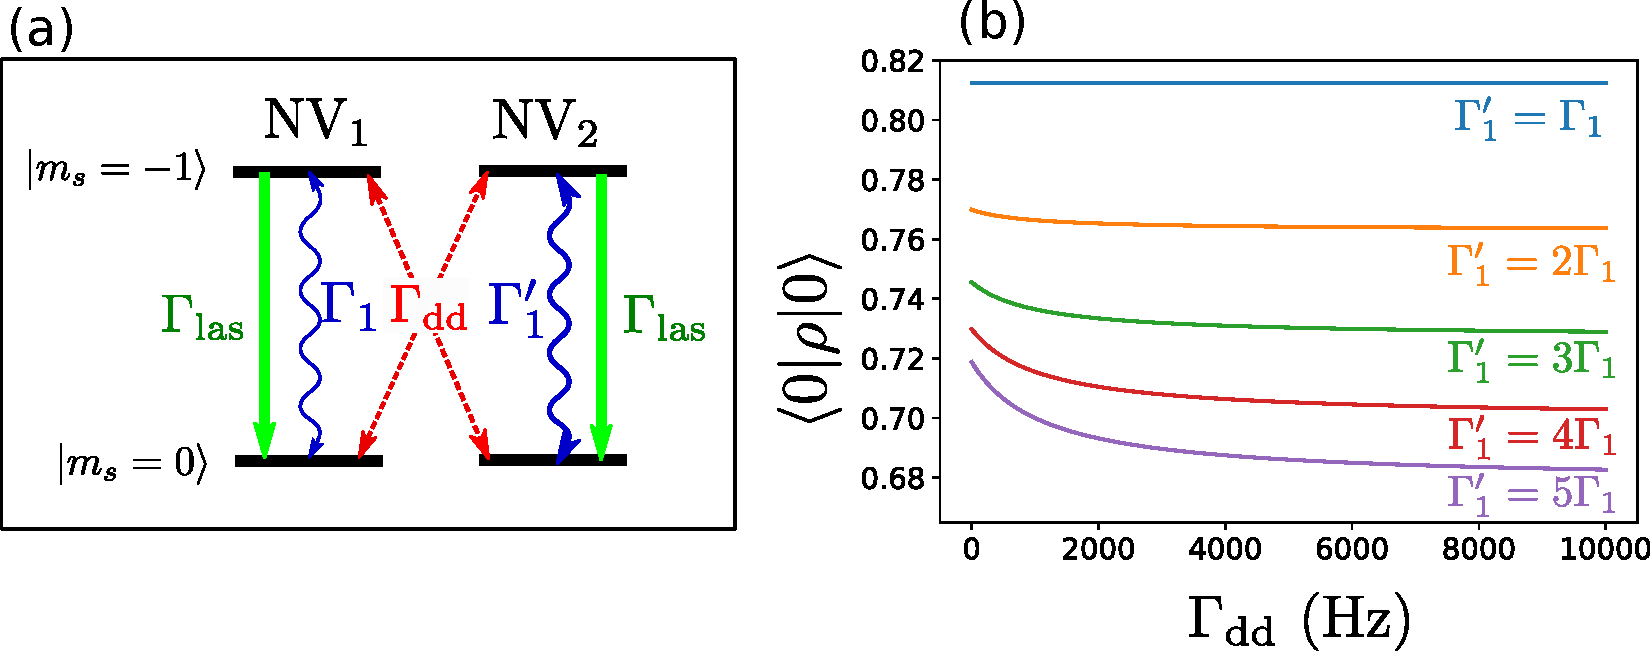
\includegraphics[width=\textwidth]{Figures/inhomogene_2_spins}
\caption{a) Schematics of the model: we consider a four level system consisting of 2 levels of 2 NV centers resonantly coupled through the flip-flop rate $\Gamma_{\rm dd}$. These two NV centers are each pumped in their respective $\ket{0}$ state via the green laser with a rate $\Gamma_{\rm las}$, and have their own relaxation rate $\Gamma_1$ and $\Gamma_1^*$ respectively. b) Average population of the two NV centers in the $\ket{0}$ state in the steady state as a function of $\Gamma_{\rm dd}$ and $\Gamma_1^*$. The steady state was computed by solving a classical rate equation where we fixed $\Gamma_{\rm las}=1000\ \rm Hz$ and $\Gamma_1=300\ \rm Hz$.}
\label{inhomogene}
\end{figure}
A likely explanation to the observed NV-NV CR is that the NV centers are not all equivalents.

Indeed, if we assume that, for instance, the relaxation rate $\Gamma_1=1/T_1$ is not strictly the same for each NV centers, but instead follows a certain distribution $\rho(\Gamma_1)$, then CR between NV centers with different $\Gamma_1$ can explain the observations in Fig. \ref{equivalent NV-NV}.

Fig. \ref{inhomogene}-a) and b) illustrates this case. Our model here consists of two (resonantly coupled) NV centers with two different relaxation rates $\Gamma_1$ and $\Gamma_1'$. To complete the model, we add the rate $\Gamma_{\rm las}$ which is the optical pumping rate from the $\ket{-1}$ to the $\ket{0}$ state of each spin, and $\Gamma_{\rm dd}$ the flip-flop rate between the two spins \footnote{We consider here a two level system instead of the full three levels of the spin 1. The choice of $\ket{-1}$ instead of $\ket{+1}$ is arbitrary.}. We only consider here the incoherent dynamics of the population, modeled with the rates reported on Fig. \ref{inhomogene}-a). Solving for the steady state of these rate equations, we can compute the final population in the $\ket{0}$ state for both spins. 

Fig. \ref{inhomogene}-b) shows the spin population in the $\ket{0}$ state of both spins, $\rho_{00}$, as a function of the flip-flop rate $\Gamma_{\rm dd}$ and for various values of $\Gamma_1'$. The first thing to notice is that, as $\Gamma_1'$ is increased,  $\rho_{00}$ decreases. This is because NV$_2$ becomes less polarized as its decay rate increases. The second thing to notice is that, when $\Gamma_1'=\Gamma_1$, i.e. when the two NV centers are truly equivalent, the flip-flop rate has no incidence on  $\rho_{00}$. However, when $\Gamma_1'>\Gamma_1$,  $\rho_{00}$ decreases when the flip-flop rate increases. Intuitively, this can be thought of as NV$_2$ acting as a polarization drain on NV$_1$. 

We can also notice that the influence of the flip-flop rate on $\rho_{00}$ increases when the difference in decay rates between NV$_1$ and NV$_2$ increases. As a result, we can suppose that a greater inhomogeneity between the NV centers would result in a stronger NV-NV cross-relaxation effect.


\subsection{Presentation of the fluctuator model}
\begin{figure}[h]
\centering
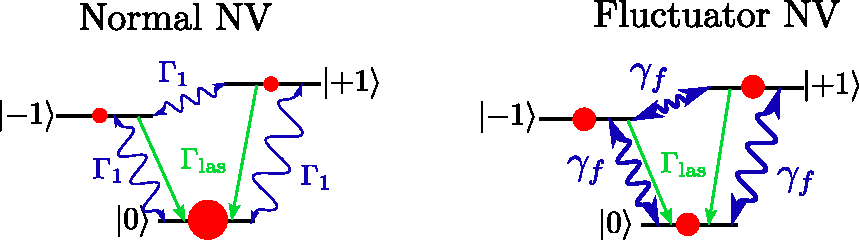
\includegraphics[width=.8\textwidth]{Figures/NV_vs_fluctuator}
\caption{Representation of a ``normal" NV center with spin depolarization rate $\Gamma_1 \ll \Gamma_{\rm las}$ and a fluctuator NV with spin depolarization rate $\gamma_f \gg \Gamma_{\rm las}$. Red circles represent the spin population in the steady state of each spin}
\label{NV vs fluct}
\end{figure}
Choi et al. in \citep{choi2017depolarization} take this approach a step further by separating the NV centers into two groups: ``normal" NV centers with a phonon-limited lifetime outside of dipole-dipole interaction, and ``fluctuators" which are NV centers with an intrinsic, extremely fast relaxation mechanism leading to a new depolarization rate $\gamma_f$. Normal and fluctuator NV are represented in Fig. \ref{NV vs fluct}: in their model, Choi et al. assume that the fluctuator decay rate is fast enough compared to the laser polarization rate $\gamma_f \gg \Gamma_{\rm las}$ that the fluctuators are effectively always depolarized. Fluctuators are therefore similar to the dark spins we introduced in the last chapter.

We should note here that, while this simplifications seem a bit extreme, the fluctuator model is more than a toy model. There are good evidence of the presence of these dark NV centers in dense NV ensemble, as will be discussed below.

In their model, the authors of \citep{choi2017depolarization} consider that the fluctuators act as a Markovian bath, meaning that the fluctuator density matrix will always read $\rho = \frac{1}{3} I$, regardless of its interaction with NV centers. With this assumption, the modification caused by the fluctuator bath on the ``normal" NV lifetimes can be analytically computed.

Other possibilities to explain the change in the relaxation rate were considered, such as spin diffusion to non-polarized NV centers (outside of the laser spot) or phonon superradiance, but they were not considered to be viable explanations: spin diffusion is orders of magnitude too slow to explain this phenomenon \citep{choi2017depolarization}, and the NV-NV CR seem to be independent of the crystal temperature \citep{jarmola2012temperature, mrozek2015longitudinal} which is incompatible with phonon superradiance \citep{choi2017depolarization}.


\subsection{Single NV center coupled to a single fluctuator}
We will follow here the notations and calculation steps in \citep{choi2017depolarization}. To compute the depolarization induced by the fluctuator bath on the NV centers, let us first consider the interaction between a single NV center and a fluctuator. Since we assume the fluctuators to be always depolarized, this step is similar to the coupling of an NV center to a dark spin done in the last chapter.

We will first decompose the dipole-dipole Hamiltonian as a product between radial and angular part:
\begin{equation}
\mathcal{H}_{\rm dd} \approx - \frac{J_0}{r^3} \left[(g+ih)(\ket{0,+1}\bra{+1,0}+\ket{0,-1}\bra{-1,0}+qS_z^1 S_z^2 \right] + h.c. ,
\end{equation}
where the expression of $J_0, g, h$ and $q$ is given in appendix [REF]. $g, h$ and $q$ are dimensionless factors that are function of the relative radial positions and orientation of the two dipoles.

We then introduce the dimensionless number $\eta$ defined as:
\begin{equation}
\label{eq eta}
\eta^2=\frac{1}{3} (\abs{g}^2+\abs{h}^2)  \frac{4\gamma_f^2}{(\omega_f - \omega_{NV})^2+4\gamma_f^2},
\end{equation}
where $\gamma_f$ is the fluctuator decay rate for each possible channel between $\ket{0}, \ket{-1}$ and $\ket{+1}$. This number $\eta$ encapsulates both the angular dependency (through $g$ and $h$) and the resonance condition between the NV center and the fluctuator.

We can note that the spectral response of a single fluctuator, for which we only consider the broadening caused by the decay rate $\gamma_f$, is a Lorentzian of half width $2\gamma_f$. This is different from the usual lifetime limited optical spectra which are Lorentzian of half width $1/2T_1=\Gamma_1/2$. The difference comes here from the fact that we consider thermalization going both ways (i.e. $\ket{e} \to \ket{g}$ and $\ket{g} \to \ket{e}$ instead of only $\ket{e} \to \ket{g}$) and that each state of the fluctuator can decay into two other states (see Fig. \ref{NV vs fluct}).

Finally, one finds that the additional depolarization rate induced by the fluctuator on the NV center reads:
\begin{equation}
\gamma_s(\mathbf{r})=\left(\frac{J_0}{r^3}\right) \frac{\eta^2}{\gamma_f}.
\end{equation}
Compared to eq. [REF], the dependency on the inhomogeneous broadening of the spins $1/T_2^*$ is hidden in the $\eta$ factor, and we have the additional broadening $\gamma_f$ coming from the fluctuators very short lifetime.

\subsection{Ensemble of NV centers coupled to a bath of fluctuators}

\begin{figure}[h]
\centering
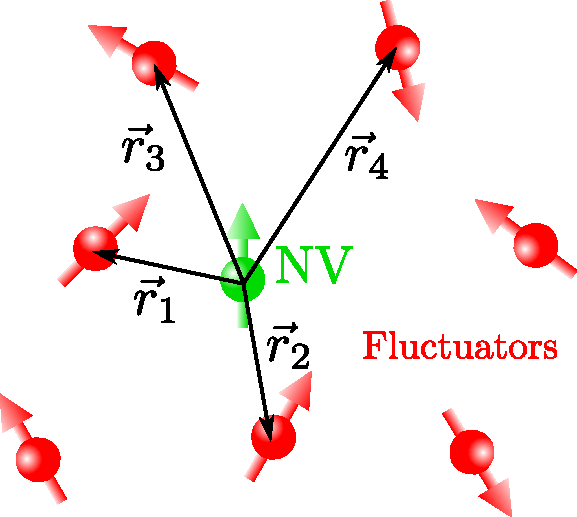
\includegraphics[width=.4\textwidth]{Figures/NV_dans_bain_fluct}
\caption{Schematics of an NV center in a fluctuator bath. The $\mathbf{r}_i$ vector represent the relative of position of fluctuator $i$ with respect to the NV center.}
\label{NV + bain fluct}
\end{figure}

The next step is to compute the depolarization caused by the ensemble of fluctuators on a single NV center.

We consider the situation pictured in Fig. \ref{NV + bain fluct}: the NV center is at the center of the frame and the position of each fluctuator is labeled $\mathbf{r}_i$. We consider that each fluctuator is an independent depolarization source, therefore the depolarization on a single NV center reads: 
\begin{equation}
\gamma=\sum_i \gamma_s(\mathbf{r}_i).
\end{equation}
We then want to compute the distribution $\rho(\gamma)$ defined as:
\begin{equation}
\rho(\gamma)=\int d\{r_i\} \rho(\{r_i\})\, \delta \left( \sum_i \gamma_s(\mathbf{r}_i) - \gamma \right).
\end{equation}
To do so, we need to determine the distribution of the fluctuators positions and orientations$\{r_i\}$. Assuming that they are homogeneously distributed in the bulk of the material, we find:
\begin{equation}
\rho(\gamma)=\frac{e^{-1/(4\gamma T)}}{\sqrt{4\pi \gamma^3 T}},
\end{equation}
where the time constant $T$ was introduced and is defined as:
\begin{equation}
\frac{1}{T}=\left(\frac{4\pi n_fJ_0\bar \eta}{3}\right)^2 \frac{\pi}{\gamma_f},
\label{eq 1/T}
\end{equation}
with $n$ the fluctuator density and $\bar \eta$ the averaged value of $\abs{\eta}$: 

\begin{equation}
\bar \eta = \int \rm{Prob}(\eta) \abs{\eta} d\eta.
\end{equation}

Finally, the polarization dynamics from the ensemble of NV centers can be computed:
\begin{equation}
P(t)=\int_0^\infty \rho(\gamma)\, e^{-\gamma t}d\gamma= e^{-\sqrt{t/T}}.
\end{equation}

In conclusion, the fluctuators causes a depolarization on the NV ensembles with a timsecale $T$ given by \ref{eq 1/T}, and the dynamics of this depolarization is that of a stretched exponential, unlike the phonon-induced depolarization which is purely exponential. 

It should be noted that the stretched exponential nature of the decay is not proper to the fluctuator model. \citep{hall2016detection} came to the same conclusion by analyzing the resonant coupling of NV centers with a P1 bath. The stretched exponential is a result from localized noise sources, randomly distributed in the bulk (3D).

\subsection{Computation of $\bar \eta$}
\label{sec computation eta}
The parameter $\bar \eta$ in eq. \ref{eq 1/T} is of crucial importance since it encompass the dependence of $1/T$ in both the magnetic field and the inhomogeneous broadening $T_2^*$ of the NV centers and the fluctuators.

We will start by separating the factor $\eta$ given in eq. \ref{eq eta} into a a geometric and a spectral part:
\begin{align}
\eta^2&=G^2(\psi_{NV},\psi_f,\theta,\phi) R^2(\omega_f,\omega_{NV}), \\
G^2&=\frac{1}{3}\left(\abs{g}^2+\abs{h}^2 \right),  \\ 
R^2(\omega_f,\omega_{NV}) &= \frac{4\gamma_f^2}{(\omega_f - \omega_{NV})^2+4\gamma_f^2}.
\end{align}

$G$ is a function which depends purely on the various angles of the problem (angles of the relative position of the NV center and the fluctuator, angle of the NV and fluctuator $z$ axis), while $R$ represents the resonance condition between the NV and the fluctuator.

We will now average this $\eta$ factor for an ensemble of fluctuators and NV centers:
\begin{align*}
\bar \eta &= \int \rm{Prob}(\eta) \abs{\eta} d\eta, \\
&= \left(\int \rho(\psi_{NV},\psi_f,\theta,\phi) |G(\psi_{NV},\psi_f,\theta,\phi)| d\psi_{NV} d\psi_f d\theta d\phi \right) \\
&\, \times \left( \int \rho(\omega_{NV}) \rho(\omega_{f}) |R(\omega_f,\omega_{NV})| d\omega_{NV} d\omega_{f} \right), \\
&= \bar G \cdot \bar R,
\end{align*}
where we introduced $\bar G$ and $\bar R$, the averaging of $|G|$ and $|R|$.

The computation of $\bar G$ will be further discussed in sec. \ref{sec quantitative T1} and in appendix [REF]. We will focus here on $\bar R$.

To perform the computation, we need to know the distributions $\rho(\omega_{NV})$ and $\rho(\omega_{f})$. We can experimentally measure $\rho(\omega_{NV})$ though ODMR, and we can reasonably expect $\rho(\omega_{f})$ to follow the same probability.

We unfortunately cannot analytically solve $\bar R$ for standard distributions of $\rho(\omega_{f})$ and $\rho(\omega_{NV})$ (either Gaussians or Lorentzians). We can however solve $\overline{R^2}$, which is relatively close to $(\bar{R})^2$ as long as $2 \gamma_f \gg 1/T_2^*$.

For a Lorentzian profile of $\rho(\omega_{f})$ and $\rho(\omega_{NV})$ defined as:
\begin{align*}
\rho(\omega_{f})&=\frac{1}{\pi \Gamma_f} \frac{1}{1+ \left(\frac{\omega_f-\omega^0_f}{\Gamma_f}\right)^2} \\
\rho(\omega_{NV})&=\frac{1}{\pi \Gamma_{NV}} \frac{1}{1+ \left(\frac{\omega_{NV}-\omega^0_{NV}}{\Gamma_{NV}}\right)^2},
\end{align*}

where $\Gamma_{f}=1/T_2^*(\rm fluctuator)$ and $\Gamma_{NV}=1/T_2^*(\rm NV)$ are the inhomogeneous broadening of the NV and fluctuator ensemble, and $\omega^0_{NV}$ and $\omega^0_{f}$ are the central angular frequencies of the NV and fluctuator ensemble. We then find that:

\begin{align*}
\overline{R^2}&= \int \rho(\omega_{NV}) \rho(\omega_{f}) \frac{4\gamma_f^2}{(\omega_f - \omega_{NV})^2+4\gamma_f^2} d\omega_{NV} d\omega_{f} \\
&=\frac{2 \gamma_f}{2 \gamma_f + \Gamma_f + \Gamma_{NV}} \cdot \frac{1}{1+\left(\frac{\omega^0_{NV}-\omega^0_{f}}{2 \gamma_f + \Gamma_f + \Gamma_{NV}}\right)^2}.
\end{align*}

In the case where $\omega^0_{NV}=\omega^0_{f}$, meaning that either the considered NVs and fluctuators are from the same class, or from two classes perfectly resonant, by substituting $\overline{R ^2}$ for $(\bar{R})^2$ (which again is only approximately valid for $2 \gamma_f \gg 1/T_2^*$) in eq. \ref{eq 1/T}, we find that:
\begin{equation}
\label{eq 1/T avec T2*}
\frac{1}{T} \propto \frac{1}{2\gamma_f + \Gamma_f + \Gamma_{NV}}.
\end{equation}

If $\rho(\omega_{f})$ and $\rho(\omega_{NV})$ follow Gaussian profiles instead, $\overline{R^2}$ is the integral of a Voigt profile, the convolution of a Lorentzian ans a Gaussian, which does not have a clear analytic solution.

Eq. \ref{eq 1/T avec T2*} is subject to several approximations: the inhomogeneous distribution of the NV centers is generally not Lorentzian, and $\overline{R^2} \neq (\bar{R})^2$ in the general case. Nevertheless, it gives us a general idea of the evolution of $1/T$ with $T_2^*$.

 \subsection{Possible microscopic origin of the fluctuators}

We should note first that a similar problem of spin ensemble relaxation rate increasing with the spin concentration was observed more than six decades ago with phosphorus doped silicon \citep{feher1959electron,honig1960electron}. It was proposed that the cause of the relaxation was the presence of fast relaxing centers coupled to the slow relaxing centers through spin diffusion \citep{honig1960electron, sugihara1963spin, yang1968concentration, vugmeister1978spin, berman2005spin}. 

This conclusion was based on previous observations on the relaxation of nuclear spins \citep{bloembergen1949interaction, de1958relaxation, blumberg1960nuclear}, where some nuclear spins had a considerably reduced lifetime due to their proximity to paramagnetic ions, and also to the resonant energy transfer between molecules \citep{forster1949experimentelle, eisenthal1964influence, yokota1967effects}, where excited donor molecules are coupled through dipole-dipole interaction to non-excited acceptors, and where the stretched exponential dynamics of the donors was first observed \citep{forster1949experimentelle}.

In the case of P-doped Si, the origin of the fast relaxing centers is thought to be closely packed P impurities, so that the electronic wavefunctions of (at least) two P centers overlap. In that case two phenomena occur: the possibility of electron tunneling, and the apparition of a contact interaction term in the dipole-dipole Hamiltonian (see appendix [REF]). Both of these phenomena could lead to fast spin relaxation, the tunneling because the spin hopping can be accompanied by a spin reversal \citep{sugihara1963spin}, and the modulation of the contact interaction strength $J$ by the crystal phonons \citep{honig1960electron}. While the non-contact dipole-dipole interaction is also modulated by the phonons, this effect would be too small to account for the fast depolarization observed here.

Similarly, \citep{choi2017depolarization} suggests that the origin of fluctuators in NV centers are closely packed NV centers or NV-impurity pairs which undergo rapid electron hopping and spin depolarization. To prove their point, they look at the charge dynamics in their sample and find that there is charge recombination in the dark with a corresponding tunneling rate between neighboring sites of $\sim 10\ \rm ns$. In contrast to P-doped Si, the NV centers are not the most abundant electronic defects in the crystal, this is why the NV$^--$N$^+$ pair in particular is thought to be a likely candidate for the fluctuators \citep{manson2018nv}.

\section{Experimental investigation of the fluctuator model}
We will now show experimental results related to the predictions of the fluctuator model.
\subsection{The stretched exponential lifetime}
\begin{figure}[h]
\centering
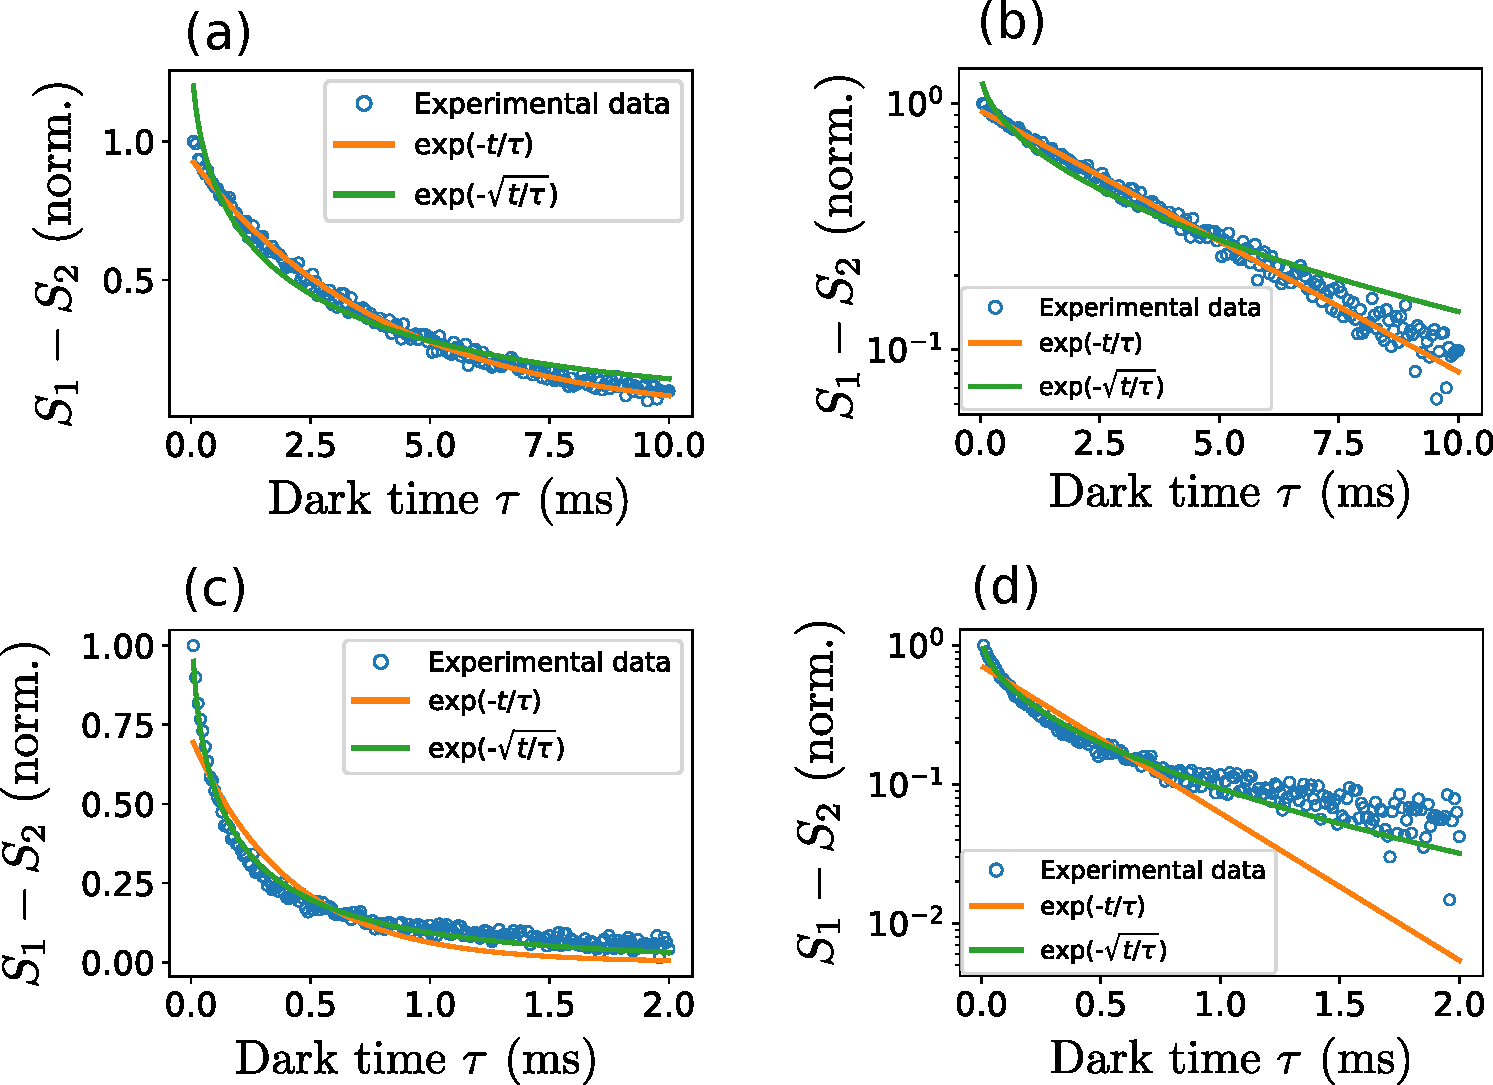
\includegraphics[width=\textwidth]{Figures/Stretch_vs_pas_stretch}
\caption{T1 measurement following the protocol described in [REF]. The best exponential and stretched exponential fits are given each time. a) Sample ADM-15-2 with B=0. The optimal $T_1$ values are $T_1^{\rm stretch}=150\ \mu \rm s$ and $T_1^{\rm exp}=410\ \mu \rm s$. b) Sample CVD-pink with B$\neq$0 and a single class probed. The optimal $T_1$ values are $T_1^{\rm stretch}=1.9\ \rm ms$ and $T_1^{\rm exp}=4.1\ \rm ms$}
\label{stretch_or_not_stretch}
\end{figure}
$T_1$ measurements with dense ensemble of NV centers and when many classes are resonant with each other (typically when B=0) indeed tend to show stretched exponential profiles.

Fig. \ref{stretch_or_not_stretch} shows an example of that: in Fig. \ref{stretch_or_not_stretch}-a) the $T_1$ measurement comes from sample ADM-15-2 at B=0. The profile is clearly better fitted by a stretched exponential than a regular exponential, and the timescale found $T_1^{\rm stretch}=150\ \mu \rm s$ is much shorter than the expected phonon limite lifetime of a few ms.

On the other hand, Fig. \ref{stretch_or_not_stretch}-b) shows a $T_1$ measurement coming from sample CVD-pink for B$\neq$0. This time the profile is more exponential, and the value $T_1^{\rm exp}=4.1\ \rm ms$ is coherent with a phonon-limited lifetime. Even though the sample CVD-pink shows some NV-NV CR feature, the spin dynamics in this sample is still dominated by the phonons, which explains the exponential profile.


\subsection{Fitting $T_1$ profile in the general case}

\begin{figure}[h]
\centering
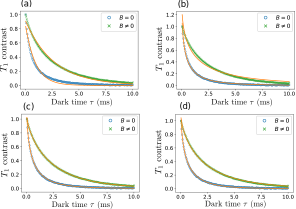
\includegraphics[width=\textwidth]{Figures/various_fit_formulae}
\caption{Different fitting procedure on two $T_1$ measurements done on sample ADM-150-1 for $B=0$ and $B\neq0$. \\ a) Exponential fit $S(\tau)=\exp (-\tau/T_1^{\rm ph})$. \\ b) Stretched exponential fit $S(\tau)=\exp (-\sqrt{\tau/T_1^{\rm dd}})$. \\ c) Bi-exponential fit $S(\tau)=\exp (-\tau/T_1^{\rm ph} -\sqrt{\tau/T_1^{\rm dd}})$. \\ d) Bi-exponential fit with fixed $T_1^{\rm ph}=5\ \rm ms$: $S(\tau)=\exp (-\tau/5 -\sqrt{\tau/T_1^{\rm dd}})$.}
\label{various_fit_formulae}
\end{figure}

\begin{table}[htbp]
\centering
\caption{Fitting parameters for Fig.
 \ref{various_fit_formulae}}
 \label{fitting table}
\begin{tabular}{c|ccc|ccc}
\toprule
Figure &  \multicolumn{3}{c}{$B=0$} & \multicolumn{3}{c}{$B\neq0$}\\
\midrule
{} &  $T_1^{\rm ph}$ (ms)& $T_1^{\rm dd}$ (ms) & $1-R^2$ &  $T_1^{\rm ph}$ (ms)& $T_1^{\rm dd}$(ms)& $1-R^2$\\
\midrule
Fig. a) & 0.95 & * & $2\cdot 10^{-2}$ & 2.64 & * & $6\cdot 10^{-3}$ \\
Fig. b) & * & 0.32 & $2\cdot 10^{-3}$& * & 1.03 & $2\cdot 10^{-2}$ \\
Fig. c) & 6.75 & 0.44 & $6\cdot 10^{-4}$ & 4.22 & 7.19 & $2\cdot 10^{-4}$\\
Fig. d) & \textbf{5} & 0.51 & $6\cdot 10^{-4}$ & \textbf{5} & 4.65 & $6\cdot 10^{-4}$\\
\bottomrule
\end{tabular}

Bold characters indicate parameters that were arbitrarily fixed.
\end{table}

For many samples however, the $T_1$ profile is neither fully exponential nor fully stretched exponential, because the relaxation time associated with CR, which we will call $T_1^{\rm dd}$ is of the same order as the phonon limited lifetime $T_1^{\rm ph}$. Sometimes the same sample can go from mostly exponential to mostly stretched exponential depending on the number of NV-NV co-resonances, forcing us to include both aspects if we want a unique fitting formula.

Fig. \ref{various_fit_formulae} shows four different fitting procedure on the two same experimental data. The data here are two $T_1$ measurements done on the same sample ADM-150-1, following the protocol described in [REF], with and without an external magnetic field ($\sim 50 G$). The magnetic field was strong enough to split the four classes and only one class was probed in the case $B\neq0$ , whereas all 4 classes were resonant in the case $B=0$, which strongly increases the NV-NV CR. 

The fits used here are either purely exponential or purely stretched exponential, or a combination of both where the exponential lifetime $T_1^{\rm ph}$ was either left as a free parameter or fixed at a value $T_1^{\rm ph}=5\ \rm ms$. The values of the different fitting parameters used is reported in Table \ref{fitting table}.

We can see that neither the purely exponential nor stretched exponential fits can be satisfying for both measurements: the $B=0$ curve is poorly fitted by the exponential fit and the $B \neq 0$ curve is poorly fitted by the stretched exponential. The protocols that include both exponential and stretched lifetimes correctly fit both curves. In the case of Fig. \ref{various_fit_formulae}-d), we arbitrarily fixed $T_1^{\rm ph}=5\ \rm ms$ since this is the value we typically measure on samples with low NV density, and we expect that the phonon-limited exponential lifetime is not modified by the NV concentration.

Since the protocol where $T_1^{\rm ph}$ was fixed and the one where it wasn't both correctly fit our data, we decided to use the protocol where $T_1^{\rm ph}$ was fixed because there is one less free parameter in the fitting function, and the values we obtain on $T_1^{\rm dd}$ can be directly compared. 

We should note however that the values of $T_1^{\rm dd}$ we obtain are not absolute. Indeed, in the case of Fig. \ref{various_fit_formulae}, the value of $T_1^{\rm ph}$ can be somewhat arbitrarily fixed between 3 and 6 ms with satisfying fits, and the resulting values $T_1^{\rm dd}$ can vary by almost an order of magnitude in the case of $B\neq0$. While this technique of measuring $T_1^{\rm dd}$ is useful to compare different cases, because it is fairly sensitive, it is not an exact measurement of the dipole-dipole induced lifetime.

\begin{figure}[h]
\centering
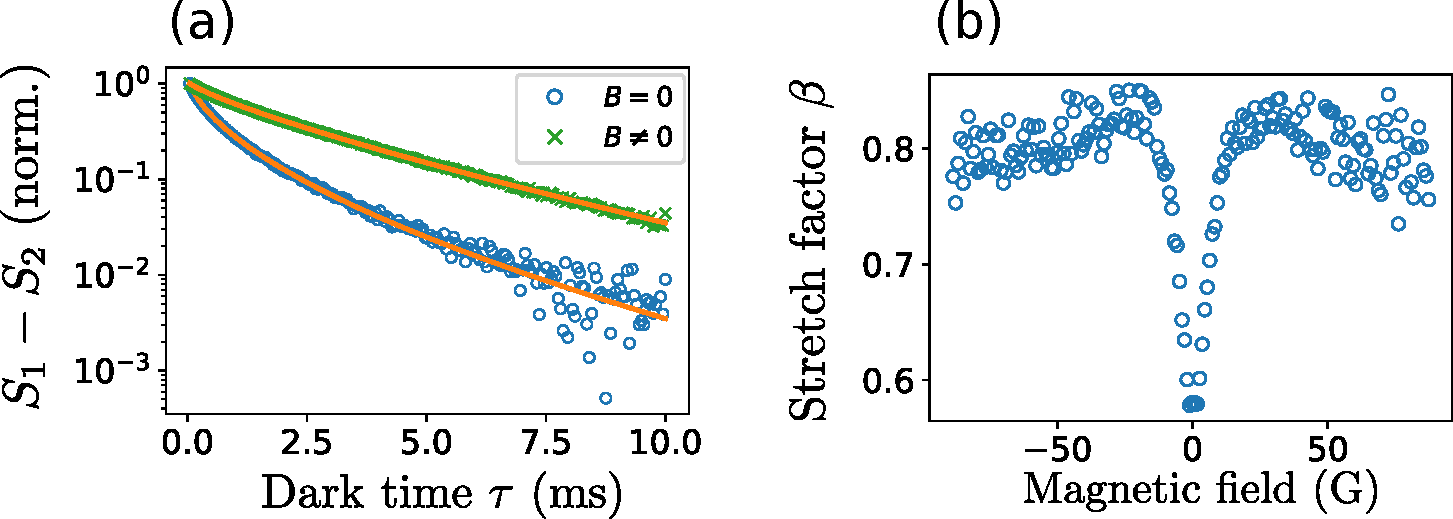
\includegraphics[width=\textwidth]{Figures/betas}
\caption{a) Same two measurements as Fig. \ref{various_fit_formulae} with the fitting formula $S(\tau)=\exp ((-\tau/T_1)^{\beta})$. The fitting parameters are $\beta=0.58$ and $T_1=0.46\ \rm ms$ for $B=0$, and $\beta=0.80$ and $T_1=2.15\ \rm ms$ for $B\neq0$. b) Optimal $\beta$ parameter found for each $T_1$ measurement as a function of the external magnetic field (still on sample ADM-150-1).}
\label{betas}
\end{figure}

Finally, another fitting procedure is shown in Fig. \ref{betas}. This time we are using a single stretched exponential with an arbitrary stretch factor $\beta$. Fig. \ref{betas}-b) shows the optimal $\beta$ parameter as a function of the external magnetic field. We can then confirm that the $T_1$ profile gets closer to a stretched exponential ($\beta=0.5$) when $B$ goes to 0. 

Even though this method also yields satisfying fits, it needs two free parameters to work ($\beta$ and $T_1$), so we decided to go with the method of Fig. \ref{various_fit_formulae}-d) instead.

\subsection{The fluctuators linewidth}

\subsubsection{The fluctuators spectral response}
\begin{figure}[h]
\centering
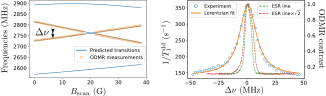
\includegraphics[width=\textwidth]{Figures/fluctuator linewidth}
\caption{Measurement of the fluctuators linewidth on sample ADM-150-2 using the same setup as in Fig. \ref{equivalent NV-NV}. a) Simulation of the $\ket{0} \to \ket{-1}$ transition frequency for the four classes of NV centers and actual frequencies of the two central classes from ODMR measurements. b) Measurement of $T_1^{\rm dd}$ as a function of the splitting $\Delta \nu$ between the two central classes, fitted with a Lorentzian of half-width $\sigma=8.8 \pm 0.2\ \rm MHz$. The green dashed line correspond to the ODMR spectrum of a single class of NV centers, and the red dashed one to the same line scaled up by a factor $\sqrt{2}$}
\label{fluct linewidth}
\end{figure}



One of the main arguments in favor of the fluctuator model is the measurement of the fluctuators spectral response. Indeed, as we will see, the fluctuator lifetime is so short that it significantly broadens the fluctuators spectral response compared to standard NV centers.

The fluctuator are effectively dark to ODMR measurement since they are not polarized, but we can measure their linewidth through CR the same way we would do for a dark spin, as detailed in \citep{hall2016detection}.

Fig. \ref{fluct linewidth} shows an experiment similar to the one presented in Fig. \ref{equivalent NV-NV}. A variable magnetic $B_{\rm scan}$ in addition to an offset magnetic field $B_{\rm DC} \sim 100\ \rm G$ are used in order to create a crossing between two classes of NV centers, but this time measuring the spin decay rate instead of the PL.

Fig. \ref{fluct linewidth}-a) shows the simulated transitions of the four classes of NV centers as a function of the magnetic field, and the experimentally measured central frequencies of the two classes of interest when the two lines can be clearly separated. Having a precise measurement of the detuning between the two classes $\Delta \nu$ is key in this experiment to get a precise value of the fluctuator linewidth.
%Because the $T_1$ measurement protocol described in [REF] requires a resonant microwave pulse with the NV probed, we specifically record ODMR spectra of their two central lines to get a precise measurement of the Larmor frequency. In the region where the two ODMR lines overlap we have to use a linear regression to get the Larmor frequency of each class.

Fig. \ref{fluct linewidth}-b) shows the dipole-dipole induced relaxation rate $\Gamma_1^{\rm dd}=1/T_1^{\rm dd}$ as a function of the detuning $\Delta \nu$ between the two central classes. For each magnetic field value, a $T_1$ profile was recorded and fitted following the procedure described in Fig. \ref{various_fit_formulae}-d) where we again fixed $T_1^{\rm ph}=5\ \rm ms$. We also show the ODMR spectrum of a single NV class for comparison.

We can clearly see that the $\Gamma^{\rm dd}$ profile is much broader than the ODMR line of the NV centers, whereas in a standard CR process, we expect the decay rate to be proportional to the spectral overlap of the two classes \citep{hall2016detection}. If we assume that both NV classes spectral response are gaussians of same width $\sigma$, then the spectral overlap between the two classes is also a gaussian of width $\sqrt{2} \sigma$. Fig. \ref{fluct linewidth}-b) also shows the ODMR line scaled by a factor $\sqrt{2}$, which is still much narrower than the $1/T_1^{\rm dd}$ line.

We attribute this broadening to the fluctuators lifetime. Another potential explanation for the broadening could be the interaction strength between the NV center and the fluctuator, but for [NV] $\sim$ 5 ppm, the average dipole-dipole coupling strength between closest NV neighbor is $\expval{\mathcal{H}_{\rm dd}} \sim 46\ \rm kHz$, which cannot explain the $\sim 4\ \rm MHz$ broadening that we observe.

\subsubsection{The fluctuators lifetime}
\begin{figure}[h]
\centering
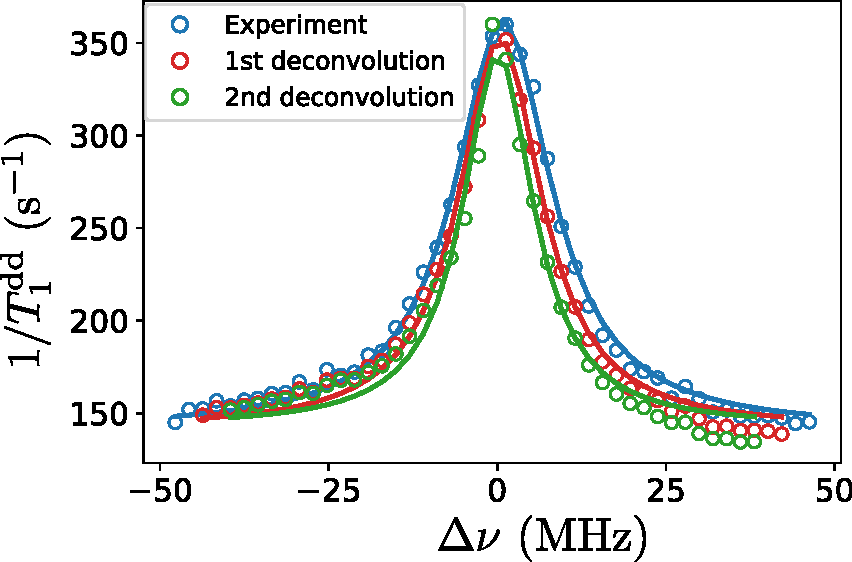
\includegraphics[width=0.6\textwidth]{Figures/deconvolution}
\caption{Blue curve $1/T_1^{\rm dd}$ data presented in Fig. \ref{fluct linewidth}. Red curve: deconvolution of the blue curve the  by the ODMR line shown on the same figure. Green curve: deconvolution of the red curve the  by the ODMR line. All three curves are fitted with Lorentzian of respective half widths $8.8 \pm 0.2$, $7.5 \pm 0.3$ and $6.4 \pm 0.4$ MHz}
\label{deconvolution}
\end{figure}

We now want to extract the fluctuators lifetime $T_1^f=1/\gamma_f$ to get further information on their potential nature. 

To do this we first assume that the dipole induced decay rate is proportional to the overlap of the spectral responses of the NV centers and fluctuators $S_{NV}$ and $S_f$. We will take $S_{NV}( \omega)$ and $S_{f}( \omega)$ as functions centered in $\omega=0$, and consider that the spectral responses are shifted by $\omega^0_{NV}$ and $\omega^0_{f}$ respectively, the central frequencies of each group. We then have:
\begin{align*}
\frac{1}{T_1^{\rm dd}} &\propto \int S_{NV} (\omega-\omega_{NV}^0) S_f (\omega-\omega_{f}^0) d\omega \\
&= \int S_{NV} (\omega-\Delta \omega) S_f (\omega)
 d\omega \\
 &= (S_{NV}*S_{f})(\Delta \omega),
\end{align*}

where $\Delta \omega=\omega_{NV}^0-\omega_{f}^0$.

Using the approximation $\bar {R ^2} \approx (\bar{R})^2$ detailed in sec. \ref{sec computation eta}, we can then decompose the fluctuator spectral response between the lifetime contribution and the inhomogeneous broadening:
\begin{equation}
S_{f}(\omega)=\left(S_f^*(\omega)\right)*\left(\frac{1}{1+\left(\frac{\omega}{2 \gamma_f}\right)^2} \right),
\end{equation}

where $S_f^*$ is the spectral broadening caused by the inhomogeneous distribution of the fluctuators, which we will suppose to be equal to $S_{NV}$. With these assumptions, we are now ready to extract $\gamma_f$ from the data of Fig. \ref{fluct linewidth}.

The first way to do this, as was done for NV-P1 CR in \citep{hall2016detection}, is to deconvolve the $1/T_1^{\rm dd}$ data by the ODMR spectrum using a Wiener deconvolution algorithm. The result of the deconvolution is shown in Fig. \ref{deconvolution}: the data is deconvolved once to get the spectral response of the fluctuator (red curve), and a second time to get only the lifetime contribution of the fluctuator (green curve). Fitting with Lorentzians, we find a final value $\Gamma_2 =2\gamma_f= (2\pi) 6.38\ \rm MHz$ which corresponds to a fluctuator lifetime $T_1^f=\frac{1}{\gamma_f}=49.9\ \rm ns$.

Another, simpler alternative is to consider that the $1/T_1^{\rm dd}$ profile is a Voigt profile given by the convolution of two Gaussians of half width at half maximum (HWHM) $f_G=\frac{\sqrt{\ln (2)}}{\pi T_2^*}$ and a Lorentzian of HWHM $f_L=\frac{2 \gamma_f}{2 \pi}$:
\begin{align*}
\Gamma_1^{\rm dd}&\propto \mathcal{G}(f_G)*(\mathcal{L}(f_L)*\mathcal{G}(f_G)) \\
&\propto \mathcal{L}(f_L)*\mathcal{G}(\sqrt{2} f_G),
\end{align*}
where $\mathcal{G}(f_G)$ and $\mathcal{L}(f_L)$ denote Gaussian and Lorentzian functions of HWHM $f_G$ and $f_L$ respectively.
We can then use the formula of a pseudo-Voigt profile which gives an approximation of the Voigt profile's HWHM $f$ as a function of $f_G$ and $f_L$ \citep{ida2000extended}:
\begin{equation}
f = [f_G^5 + 2.69269 f_G^4 f_L + 2.42843 f_G^3 f_L^2 + 4.47163 f_G^2 f_L^3 + 0.07842 f_G f_L^4 + f_L^5]^{1/5}.
\end{equation}

With $f=8.78\ \rm MHz$ and $\sqrt{2}f_G=4.33\ \rm MHz$, we find $f_L=6.54\ \rm MHz$ for a final lifetime value $T_1^f = 48.7\ \rm ns$, a value consistent with the one found with the deconvolution method.

Doing similar calculations, \citep{choi2017depolarization} found $\gamma_f=1/T_1^f=(2\pi) 3.3\ \rm MHz$ which gives them a fluctuator lifetime value $T_1^f = 48.2\ \rm ns$, a value surprisingly similar to the one we got.


\section{Resonance between several NV classes}

The main tool to probe NV-NV CR is to use the co-resonances between the NV classes. While it is not possible to completely shut down the CR, because the NV centers from the same class are always resonant with each other, we can tune the density of resonant NV centers (and supposedly resonant fluctuators) by a factor of 4 by playing with the inter-class co-resonances. We will discuss here the various scenarios where NV classes overlap, and the quantitative impact it has on the centers' spin $T_1$.

\subsection{Geometric conditions for inter-class resonance}

\begin{figure}[h!]
\centering
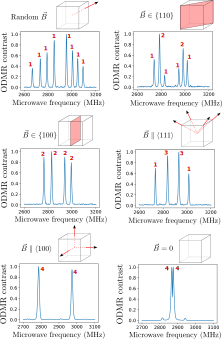
\includegraphics[width=0.8\textwidth]{Figures/Resonance_geometries}
\caption{ODMR spectra on sample ADM-15-3 as a function of the magnetic field orientation. The field amplitude is $\sim 60\ \rm G$. Red numbers represent the number of resonant classes for each ODMR line. The cubes represent the diamond unit cell, and the red planes/arrow the possible orientations of the magnetic field}
\label{ODMR_geometries}
\end{figure}

There are four possibilities to obtain inter-class resonance (outside of the non-equivalent CR discussed in sec. \ref{non_equi_valent_CR}). These possibilities are:
\begin{itemize}
\item $\mathbf{B} \in \{110\}$. We refer by $\{110\}$ as any plane orthogonal to a $\langle 110 \rangle$ or equivalent direction. In this magnetic configuration, two classes are at resonance and the two other ones are spectrally isolated.
\item $\mathbf{B} \in \{100\}$. In this magnetic configuration, the four classes form two pairs of co-resonance.
\item $\mathbf{B} \parallel \langle 111 \rangle$. In this configuration discussed in the last chapter, one class is aligned with the magnetic field and is spectrally isolated while the three other form a resonant triplet.
\item $\mathbf{B} \parallel \langle 100 \rangle$. In this configuration also discussed in the last chapter, the four classes are resonant.
\end{itemize}
We should add to this list the case $\mathbf{B}=0$ where all four classes are also resonant, and any other possibility (which I will call random $\mathbf{B}$) where all four classes are spectrally separated. 

An ODMR spectrum and a representation of the magnetic field in the diamond unit cell for each of these six possibilities is shown in Fig. \ref{ODMR_geometries}.

\begin{figure}[h]
\centering
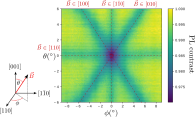
\includegraphics[width=\textwidth]{Figures/carte}
\caption{PL contrast as a function of the magnetic field polar and azimuthal angle with respect to the [100] axis on sample CVD-pink. The field amplitude is $\abs{B} \sim 115 G$. The locus of the magnetic field in specific planes is noted by red dashed lines.}
\label{Carte}
\end{figure}

This relation between NV-NV class resonances and the magnetic field being in specific crystalline planes or directions means that we can determine the crystal main axes simply by PL experiments.

Fig. \ref{Carte} shows a map where we simply monitored the PL of sample CVD-pink while scanning the magnetic field angle around the [001] axis, thanks to a permanent magnet on a motorized goniometer. We have also reported the locus of $\mathbf{B}$ being in the planes [100], [010], [110] and [$1\bar 1 0$].

We know that when $\mathbf{B}$ belongs to any of these four planes, there is a co-resonance between at least two NV classes. This co-resonance leads to an increase in NV-NV CR and a faster depolarization of the spins involved, which ultimately leads to a drop in PL. We can indeed see in fig. \ref{Carte} that there is clear correlation between the loci of $\mathbf{B}$ and drops in PL. We can also see that the PL is at its lowest when $\mathbf{B}\parallel [001]$, which corresponds to a four class degeneracy.

\subsection{Quantitative modification of $T_1$}
\label{sec quantitative T1}
\begin{table}[htbp]
\centering
\caption{Theoretical and experimental values of $\Gamma_1^{\rm dd}=1/T_1^{\rm dd}$ for various magnetic field configurations, expressed as a function of the value found for an isolated class. The experimental values were measured on sample ADM-15-3 using the protocol of Fig. \ref{various_fit_formulae}-d) with $T_1^{\rm ph}= 5\ \rm ms$.}
 \label{T1 champ mag}
\begin{tabular}{c|cc}
\toprule
$\Gamma_1^{\rm dd} (\mathbf{B})$ &  Theory & Experimental \\
\midrule
random $\mathbf{B}$ (1 class) & $\Gamma_0^{\rm th}$ & $1.53\pm 0.04$ ms$^{-1} \equiv \Gamma_0^{\rm exp}$ \\
$\mathbf{B} \in \{110\}$ (2 classes) & 10.0 $\Gamma_0^{\rm th}$ & $5.2 \pm 0.1$ $\Gamma_0^{\rm exp}$ \\
$\mathbf{B} \in \{100\}$ (2 classes) & 7.24 $\Gamma_0^{\rm th}$ & $4.2 \pm 0.1$ $\Gamma_0^{\rm exp}$ \\
$\mathbf{B} \parallel \langle 111 \rangle$ (3 classes) & 28.4 $\Gamma_0^{\rm th}$ & $11.6 \pm 0.4$ $\Gamma_0^{\rm exp}$ \\
$\mathbf{B} \parallel \langle 100 \rangle$ (4 classes) & 42.8 $\Gamma_0^{\rm th}$ & $14.1 \pm 0.5$ $\Gamma_0^{\rm exp}$ \\
$\mathbf{B}=0$ (4 classes) & 51+($^*$) $\Gamma_0^{\rm th}$ & $19.9 \pm 0.8$ $\Gamma_0^{\rm exp}$ \\
\bottomrule
\end{tabular}

($^*$) The case $\mathbf{B}=0$ will be detailed in the next chapter. The theoretical value is a lower bond.
\end{table}

The fluctuator model allows quantitative predictions of the change in the spin lifetime, thanks to eq. \ref{eq 1/T}. There are however several unknown in this equation, such as the fluctuator density and lifetime which can be hard to estimate. It is however relatively easy to compare the predictions of eq. \ref{eq 1/T} for various magnetic field configurations.

What we decided to do was to take the case of an isolated class, where we consider that NV centers from said class or only affected by fluctuators of the same class, as the baseline value for the dipole-dipole decay rate $\Gamma_0$, and to express the decay rates when 2, 3 or 4 classes are co-resonant as a function of $\Gamma_0$. Doing so allows to normalize $n_f$ and $\gamma_f$ in eq. \ref{eq 1/T} and to keep $\bar G$ the geometrical part of $\bar \eta$ as the only unknown.

$\bar G$ can be analytically or numerically computed for each of the magnetic configurations listed before, as detailed in appendix [REF]. This allows us to predict the value of the spin decay rate in every situations as a function of the decay rate of an isolated class.

Table \ref{T1 champ mag} shows these predicted values, along with experimental ones on sample ADM-15-3. The experimental values were obtained with the protocol described in Fig. \ref{various_fit_formulae}-d) with a double exponential fit where we fixed again $T_1^{\rm dd}=5\ \rm ms$.

The theoretical values are in a good qualitative agreement with the experimental ones, both ranking the different scenarios in the same order. The quantitative predictions of the theory however are rather poor, being off by more than a factor of 3 for the shortest lifetimes.

It should be noted that the experimental values were heavily influenced by the choice of the parameter $T_1^{\rm ph}$. Using for example $T_1^{\rm ph}=2.5\ \rm ms$ gave results closer to the theoretical ones. Nevertheless, the fluctuator model generally tends to overestimate the depolarization rates.The authors of \citep{choi2017depolarization} for instance found that a 2-class degeneracy (the authors did not precise whether this was a $\mathbf{B} \in \{110\}$ or $\mathbf{B} \in \{100\}$ configuration) yielded an increased depolarization rate by a factor $\sim 4$, a value comparable to the one we found in table \ref{T1 champ mag}, and two times smaller than the predicted one. We can also see in Fig. \ref{fluct linewidth} that a $\mathbf{B} \in \{110\}$ configuration leads to a $\sim 2.5$ times increase in $\Gamma_1^{\rm dd}$, 4 times smaller than the predicted factor of 10.

The failure of the fluctuator model to accurately predict the changes in $T_1$ is one of the reasons that led us to believe that the model is incomplete.

\section{Conclusion and perspectives}

In conclusion, we have seen in this chapter that dense NV ensemble present ``anormal" CR between the NV centers, and we have shown how the fluctuator model developed by Choi et al. in \citep{choi2017depolarization} can explain this behavior. The fluctuator model not only explains the NV-NV CR, but also correctly predicts the stretched exponential lifetime profile. It also correctly predicts that the fluctuators have a broader spectral response than the other NV centers. Nevertheless, the model does not describe perfectly every aspects of NV-NV relaxation, and there still are many aspects of this problem, both theoretical and experimental, to explore.

In what follows I will describe what I think would be interesting investigation points to further understand the NV-NV relaxation and the fluctuator model.

\subsection{Limitations of the fluctuator model}
\begin{figure}[h]
\centering
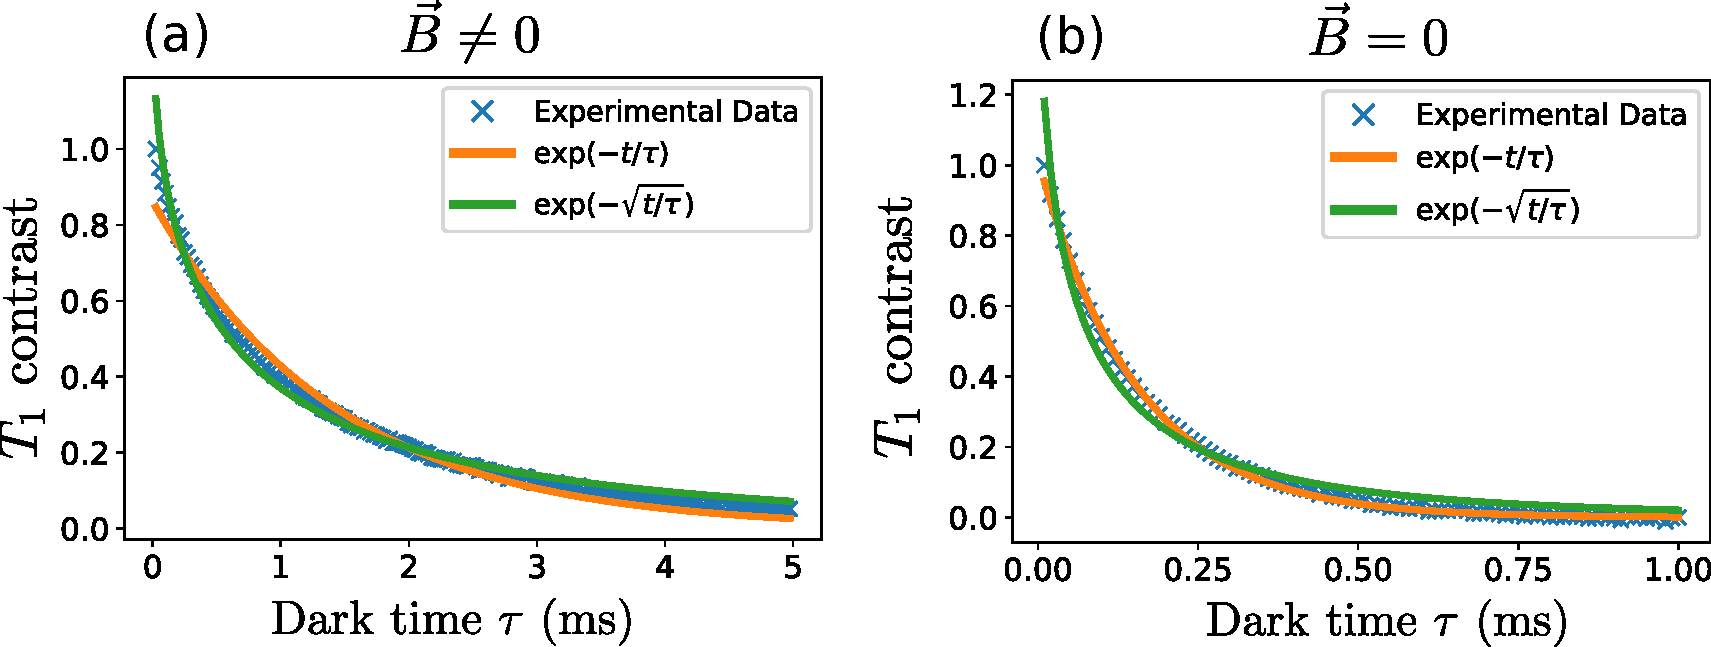
\includegraphics[width=\textwidth]{Figures/Anormal_T1}
\caption{$T_1$ measurements on sample ADM-15-4, fitted with pure exponential or stretched exponential. a) $T_1$ of a single isolated class when $\mathbf{B} \neq 0$. The optimal fit parameters are respectively $T_1^{\rm exp}=1.43\ \rm ms$ and $T_1^{\rm stretch}=0.56\ \rm ms$. b) $T_1$ of the four degenerate classes when $\mathbf{B}=0$. The optimal fit parameters are respectively $T_1^{\rm exp}=0.15\ \rm ms$ and $T_1^{\rm stretch}=0.05\ \rm ms$.}
\label{anormal T1}
\end{figure}

I already mentioned that the discrepancy between the theoretical and experimental $T_1$  values were an issue of the current fluctuator model, although the difference could come in part from the $T_1$ fitting procedure. Another, more glaring problem is the fact that some $T_1$ profile are not stretched exponential.

Fig. \ref{anormal T1} shows $T_1$ measurement on sample ADM-15-4, either on a single isolated class ,where the dipole-dipole interactions are at their weakest, or on all four resonant classes at $\mathbf{B}=0$, where the interactions are at their strongest.

For the single isolated class, the $T_1$ profile seems to be closer to a stretch exponential, which is coherent with the fact that the lifetime $T_1 \sim 1\ \rm ms$ is already smaller than the expected phonon limited lifetime $T_1^{\rm ph} \sim 5\ \rm ms$. However when $\mathbf{B}=0$, although the lifetime gets $\sim$ 10 times shorter, the profile becomes clearly exponential. 

The spin dynamics in this sample is still dominated by resonant dipole-dipole interactions: the more classes are brought to resonance, the shorter the spin $T_1$. But here, the profile gets closer to a pure exponential when $T_1$ decreases, which is in complete contradiction with the fluctuator model.

This particular sample was a 15 $\mu$m micro-diamond, which could have a role in this observation since we know that spins near the surface have a reduced $T_1$ \citep{rosskopf2014investigation}, and micro-diamonds have proportionally more near surface spins. But other diamonds from the same batch, such as the one measured in Fig. \ref{stretch_or_not_stretch}, show clearly stretched exponential profile in the same conditions, and meanwhile some bulk diamonds show very short non-stretched exponential lifetimes, similar to the present sample.

It seems therefore that the current fluctuator model does not correctly describe the spin dynamics of every NV-dense samples. Looking at what was previously done for P-doped SI \citep{vugmeister1978spin} or for resonant energy transfer between molecules \citep{yokota1967effects}, the fluctuator model could probably be improved by taking into account the finite lifetime of the fluctuators (i.e. the saturation of the NV-fluctuator CR), and the spin diffusion between NV centers (the fluctuator model only considers NV-fluctator interactions and not NV-NV interactions).

\subsection{Investigation of the fluctuators nature}
While the hypothesis of fluctuators being clusters of NV centers or NV-other spins is solidified by the precedents in P-doped Si \citep{honig1960electron} or F centers in KCl \citep{warren1964spin}, there are still many unknowns on the exact nature of the fluctuators. There are at least two aspects that I think merit to be investigated.

The first one would be to study the fluctuator spectral profile on various samples showing NV-NV CR. In particular it would be interesting to know whether this profile is always Lorentzian, and what its linewidth is. In the sample I studied on Fig. \ref{fluct linewidth}, I found a value for $\gamma_f$ surprisingly similar to the one found in \citep{choi2017depolarization}, even tough my sample only had $[\rm NV] \sim 3 ppm$ compared to the $[\rm NV] \sim 45 ppm$ sample used in \citep{choi2017depolarization}. If $\gamma_f$ was found to be somewhat of a constant among all samples showing NV-NV CR, this would give us a lot of information on the potential nature of the fluctuators. Studying the temperature dependency of $\gamma_f$ could also give us information on whether the depolarization mechanism is due to tunneling or modulation of the $J-$coupling by the phonons.

The other aspect would be to identify potential defects that could form fluctuators when paired with NV centers. The main candidate for this would be substitutional nitrogen (P1 or P1$^+$ centers) since they are the most abundant electronic spin species in the diamond we use. The ideal way to confirm this hypothesis would be to compare the spin $T_1$ for  different samples with the same [NV] concentration, but different [P1] concentration. If indeed P1 centers play a role in the presence of fluctuators, we would expect a shorter NV $T_1$ time in the sample with high P1 concentration.


\printbibliography
\end{document}